\chapter{Cách thức hoạt động của blockchain}
\comment{
\section{Mật mã Chìa Khóa Bất đối xứng}

Mật mã bất đối xứng (Asymmetric cryptography), hay còn gọi là mật mã công cộng (public cryptography) là một thành phàn nền tàng của blockchain và các loại tiền ảo như Bitcoin và Ethereum. Những kỹ thuật mật mã nâng cao này đảm bảo rằng nguồn gốc của giao dịch là hợp lệ và các tin tặc không thể đánh cắp tiền của người dùng.

\subsection{Khái niệm}
Mật mã bất đối xứng luôn sử dụng hai chìa khóa: văn bản được mã hóa bằng một trong hai chìa khóa chỉ có thể được giải mã với chìa khóa kia, và ngược lại. Khi sử dụng mật mã bất đối xứng trong thực tế, các chìa khóa này được gọi là chìa khóa công cộng và chìa khóa riêng tư để làm nổi bật vai trò của chúng. Chìa khóa công cộng đựoc chia sẽ cho mọi người, trong khi chìa khóa riêng tư được giữ bí mật.  Vì lí do này, mật mã bất đối xứng còn được gọi là mật mã chìa khóa công cộng - riêng tư.

Hai trường hợp sử dụng cơ bản của chìa khóa công cộng và cổ điển là:

\begin{itemize}
	\item Mọi người đều có thể sử dụng chìa khóa công cộng để mã hóa dữ liệu mà say đó chỉ có thể được giải mã bởi người nám giữ chìa khóa riêng tư tương ứng. Điều này tương đồng với một hộp thư công cộng nơi mọi người có thể cho thư vào nhưng chỉ có chủ sở hữu có thể mở nó.
	\item Người nắm giữ chìa khóa riêng tư có thể sử dụng nó để mã hóa sử dụng dữ liệu mà sau đó chỉ có thể được giải mã bởi những người sở hữu chìa khóa công cộng tương ứng, Điều này tương đồng với một bảng thông báo công cộng nơi những ai có bản sao chép của chìa khóa công cộng có thể đọc tin nhắn nhưng chỉ người nắm giữ chìa khóa riêng tư có thể tạo ra tin nhắn
\end{itemize}

Blockchain sử dụng mật mã bất đối xứng nhằm đạt được hai mục địch:
\begin{itemize}
	\item Xác định tài khoản: Tài khoản người sư dụng là chìa khóa mật mã công cộng.
	\item Xác thực giao dịch: Chủ sở hữu của tài khoản, người nằm giữ quyền sở hữu tài sản, tạo ra một văn bản được mã hóa với chìa khóa riêng tư tương ứng. Văn bản được mã hóa này có thể được chứng thực bằng cách sử dụng chìa khóa công cộng tương ứng, chính là số tài khoản chủ sở hữu.
\end{itemize}

\section{Chữ ký điện tử}

Trong thế giới thực, chữ ký viết tay trên văn bản tuyên bố sự đồng thuận của tác giả với nội dung của văn bản đã ký. Khả năng chứng minh của chữ ký bằng nay dựa trên sự độc nhất của chữ  viết tay của mỗi người.

Chữ ký điện tử là phiên bản điện tử tương đờng của chữ ký viết tay, Nó phục vụ hai mục đích:
\begin{itemize}
	\item Xác thực tác giả duy nhất
	\item Tuyên bố sự đồng thuận của tác giả với nội dung văn bản và xác thực những điều được thực thi trong đó.
\end{itemize}

Trong blockchain, chữ ký điện tử của các giao dịch chính là mã băm mật mã của dữ liệu giao dịch được mã hóa bằng chìa khóa riêng tư tương ứng với tài khoản người nắm quyền sở hữu. 


\subsection{Khái niệm mã băm}
Nói một cách đơn giản, băm nghĩa là lấy một chuỗi đầu vào với độ dài bất kỳ và cho đầu ra là một chuỗi với độ dài cố định. Trong phạm vi tiền ảo như Bitcoin, các giao dịch được lấy làm đầu vào và chạy qua một thuật toán băm (Bitcoin sử dụng SHA-256) cho một đầu ra là chuỗi có độ dài cố định.
Ta có ví dụ như bảng 3.1. 

Trong trường hợp của SHA-256, bất kể đầu vào có lớn hay nhỏ đến đâu, đầu ra sẽ luôn có độ dài cố định 245-bit. Điều này trở nên quan trọng khi ngày nay, khối lượng dữ liệu và giao dịch cần xử lý ngày một lớn dần. Do đó, thay vì phải nhớ dữ liệu đầu vào, ta chỉ cần nhớ mã hash của nó để tiện theo dõi.

\subsection{Hàm băm mật mã học}
Hàm băm mật mã học (cryptographic hash function) là một lớp đặc biệt của hàm băm. Nó csubó những tính chất khác nhau khiến nó trở nên lý tướng để áp dụng trong lĩnh vực mã hóa.  

Một hàm băm mật mã học lý tưởng có những tính chất chính sau:
%Tất định: các tin nhắn giống nhau luôn có cùng mã băm.
%Nhanh chóng tính ra mã băm với mọi tin nhắn được cung cấp.
%Không thể tạo lại tin nhắn từ mã băm của nó, ngoại trừ bằng cách thử mọi tin nhắn khả dĩ
%Một thay đổi nhỏ trong tin nhắn cũng dẫn đến thay đổi mã băm của nó một cách sâu rộng, dẫn đến mã băm mới không có tương quan gì sao với mã băm cũ.
% Không thể tìm được hai tin nhắn khác nhau có cùng mã băm.


\textbf{Tính chất 1: Tất định}

Các tin nhắn giống nhau luôn có cùng mã băm.

\textbf{Tính chất 2: Tính nhanh}

Hàm băm phải có khả năng đưa ra mã hash của đầu vào một cách nhanh chóng. Nếu tiến trình không đủ nhanh thì hệ thống sẽ không hiệu quả

\textbf{Tính chất 3: Pre-Image Resistance}

Tính chất này nói rằng nếu được cho trước mã hash h, sẽ rất khó khăn để tìm được tin nhắn m thỏa h = hash(m). Khái niệm này liên quan đến tính chất của hàm một chiều.

\textbf{Tính chất 4: Thay Đổi Nhỏ ở Đầu Vào Dẫn Đến Thay Đổi Toàn Bộ Mã Hash}

Kể cả nếu ta chỉ gây một thay đổi nhỏ ở đầu vào, thay đổi được phản ánh ở mã hash mới sẽ rất lớn. Ví dụ sử dụng SHA-256:

%\begin{table}[h!]
%	\begin{tabu} to\linewidth{ |X[2] | X[8] | }
%		\hline
%		Input & Hash \\
%		\hline
%		This is a test & \seqsplit{C7BE1ED902FB8DD4D48997C6452F5D7E509FBCDBE2808B16BCF4EDCE4C07D14E} \\ \hline
%		this is a test & \seqsplit{2E99758548972A8E8822AD47FA1017FF72F06F3FF6A016851F45C398732BC50C} \\ \hline
%		
%	\end{tabu}
%	\centering
%	
%	\caption[Table caption text]{Ví dụ tác động của thay đổi đầu vào}
%\end{table}

Đây là một tính chất quan trọng vì nó sẽ dẫn đến một trong những đặc tính quan trọng nhất của blockchain, tính không thể thay đổi.

\textbf{Tính chất 5: Collision Resistant}

Một xung đột xảy ra khi hai đầu vào khác nhau tạo ra cùng một đầu ra. Một hàm băm H có tính khá xung đột nếu không ai có thể tìm được một xung. Biểu đạt một cách hình thức thì:

Một hàm băm H được cho là kháng xung đột nếu như khó khả thi để tìm hai giá trị, x và y,  với x $\neq$ y sao cho H(x) = H(y)

%Ta nói rằng "không ai có thể tìm được" một xung đột, nhưng ta không nói rằng không có xung đột nào tồn tại. Thực tế, xung đột tồn tại trong bất cứ hàm băm nào, 

 \begin{figure}[h]
	\centering	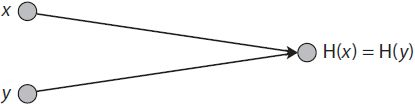
\includegraphics[width=0.9\textwidth]{collision}
	\caption{Một xung đột hàm băm, x và y là hai giá trị khác biệt, nhưng khi truyền vào hàm băm H, chúng tạo ra cùng đầu ra}
\end{figure}

\textbf{Tính chất 6: Puzzle friendliness}

Một hàm băm H được cho là puzzle friendly nếu với mọi giá trị đầu ra y, nếu k được chọn là một phân phối với  high min-entropy, khó khả thi để tìm được một đầu ra x thỏa H(k|x) = y.


% \section{Mã hóa}
% \subsection{Mật mã đối xứng}
% Với mật mã đối xứng (hoặc mã hóa chìa khóa-đồng bộ), cùng một chìa khóa được sử dụng cho cả quá trình mã hóa và giải như được thể hiện trong hình 
%
% Mật mã đối xứng có hai loại
% Stream Ciphers.
% Block Ciphers.
%
% Stream Ciphers
% Stream Ciphers nghĩa là sử dụng một chìa khóa có độ dài cố định nhằm thay thế tin nhắn với một chuỗi kí tự giả ngẫu nhiên (pseudorandom). Về cơ bản, nó mã hóa từng chữ cái của tin nhắn .
%
% 3 dạng của stream ciphers:
%
% One-time pad với bảng chữ cái
% Để thực hiện dạng mã hóa này cần có một chìa khóa có cùng số kí tự với tin nhắn và nó chỉ có thể được sử dụng một lần duy nhất.
%
% GIả sử A  gửi tin nhắn “MEET ME OUTSIDE” đến Bob. Nhưng A không muốn ai chặn tin nhắn của họ. Vì vậy, A và Bob quyết định sử dụng một one-time pad 
%
%
% Quá trình mã hóa

\subsection{Mật mã bất đối xứng}

mã hóa bất đối xứng, sử dụng một cặp chìa khóa có liên quan với nhau về mặt toán học, một chìa công khai dùng để mã hoá (public key) và một chìa bí mật dùng để giải mã (private key) như hình \ref{fig:asymmetric}. Một thông điệp sau khi được mã hóa bởi chìa công khai sẽ chỉ có thể được giải mã với chìa bí mật tương ứng. Do các thuật toán loại này sử dụng một chìa khóa công khai (không bí mật) nên còn có tên gọi khác là public-key cryptography (thuật toán mã hóa dùng chìa khóa công khai).
 \begin{figure}[ht]
	\centering
	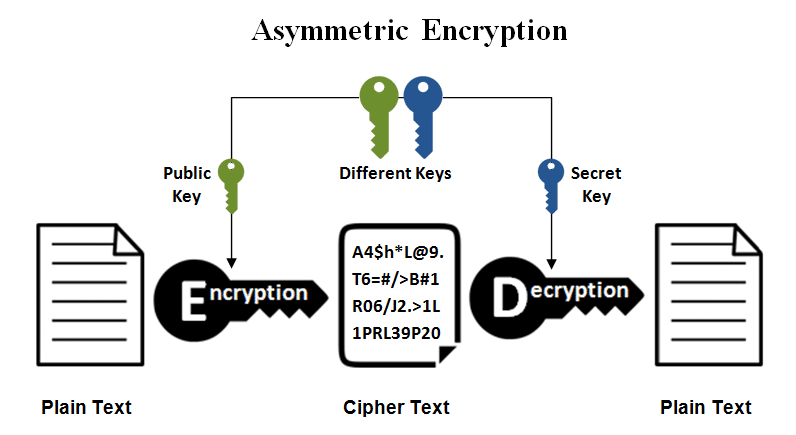
\includegraphics[width=0.9\linewidth]{image/asymmetric_cryptography}\label{fig:asymmetric}
	\caption{Minh họa mật mã bất đối xứng}
\end{figure}


Mật mã bất đối xứng có hai ứng dụng thực tế là:
Thuật toán Rivest-Shamir-Adleman (RSA).
Elliptical Curve Cryptography.}

\section{Mật mã trong blockchain}
Mật mã học là những phương pháp giúp che giấu và lộ diện, hay còn gọi là mã hóa và giải mã, thông tin thông qua các phương pháp toán học phức tạp. Điều này có nghĩa là thông tin không thể được xem bởi bất kỳ ai ngoại trừ  những người nhận được định trước. Các phương pháp bao gồm lấy các thông tin chưa được mã hóa như một đoạn văn bản, và mã hóa nó bằng cách sử dụng một thuật toán (tiếng Anh gọi là cypher).
Nó tạo nên một văn bản đã mã hóa (ciphetext), một mẩu thông tin hoàn toàn vô dụng và vô nghĩa chi đến khi được giải mã. Phương pháp mã hóa này được gọi là mã hóa chìa khóa đối xứng (symmetric-key cryptography).

Một ví dụ về mật mã xuất hiện sớm trên thế giới là mật mã Caesar (Caesar cipher), được sử dụng bởi Julius Caesar để bảo vệ các bí mật quan sự  của Roman. Mỗi chữ  cái trong một tin nhắn được thay thế với chữ cái đứng trước nó 3 chữ cái về phía bên trái trong bảng chữ cái, thông tin này về cơ bản chính là chìa khóa để giải mã tin nhắn. Các tướng của Caesar biết rằng để giải (decode) các chữ cái họ chỉ phải dịch mỗi chữ về phía phải (bảng chữ cái) ba lần, trong khi thông tin sẽ được giữ an toàn nếu bị chặn bởi kẻ thù của Caesar. Mật mã học hiện đại hoạt động tương tự, nhưng với độ phức tạp cao hơn rất nhiều.

 \begin{figure}[ht]
	\centering
	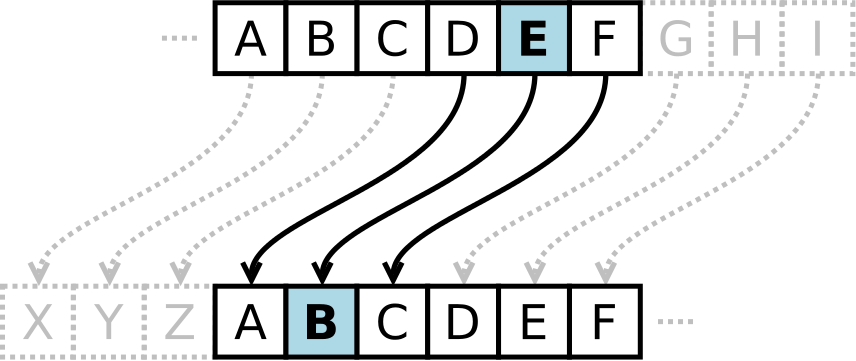
\includegraphics[width=0.9\linewidth]{image/Caesar_cipher_left_shift_of_3}\label{fig:Caesar}
	\caption{Cách thức hoạt động của một mật mã Caesar là thay thế mỗi chữ cái với một chữ khác cách một khoảng cố định trên bảng chữ cái}
\end{figure}

 \begin{figure}[ht]
	\centering
	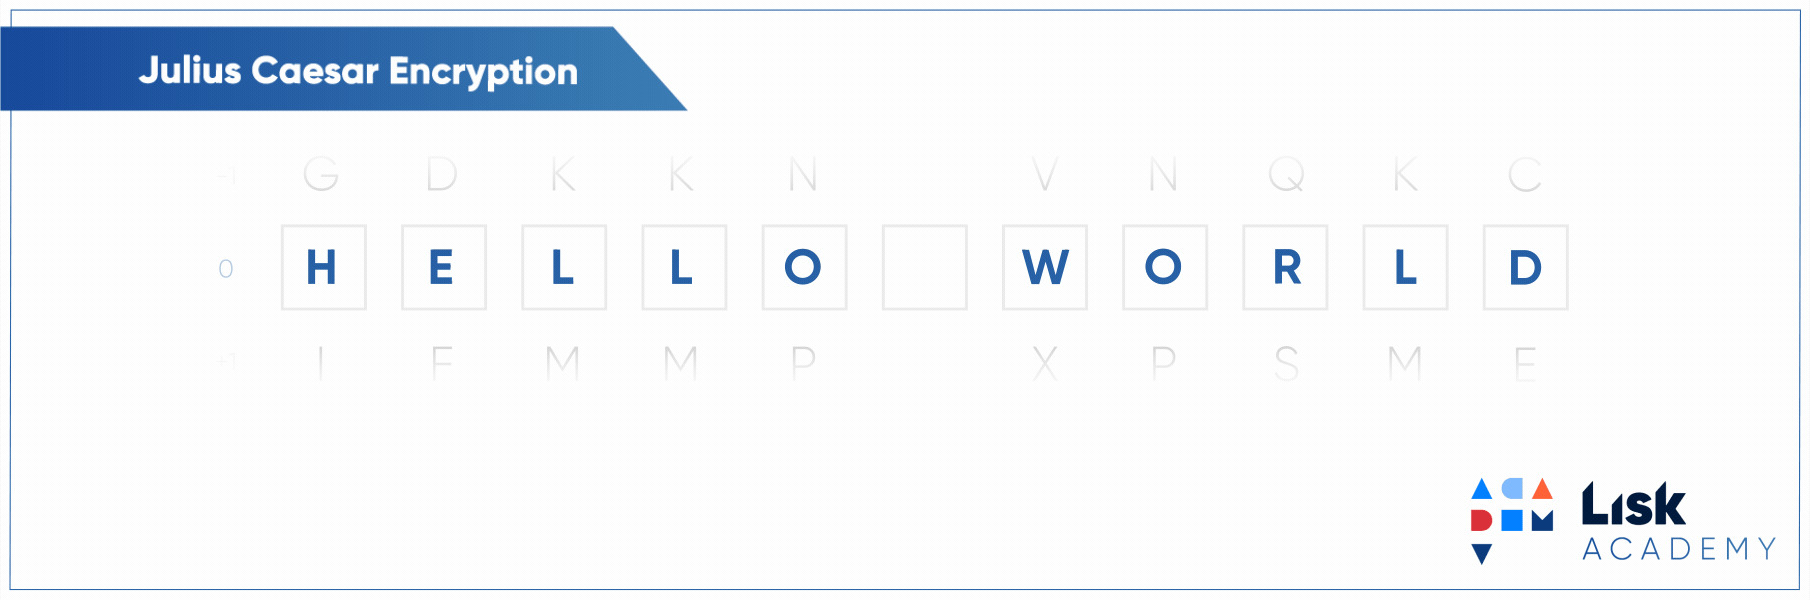
\includegraphics[width=0.9\linewidth]{image/caesarBefore}\label{fig:CaesarBefore}
	\caption{Câu "Hello World" trước khi mã hóa}
\end{figure}

\begin{figure}[ht]
	\centering
	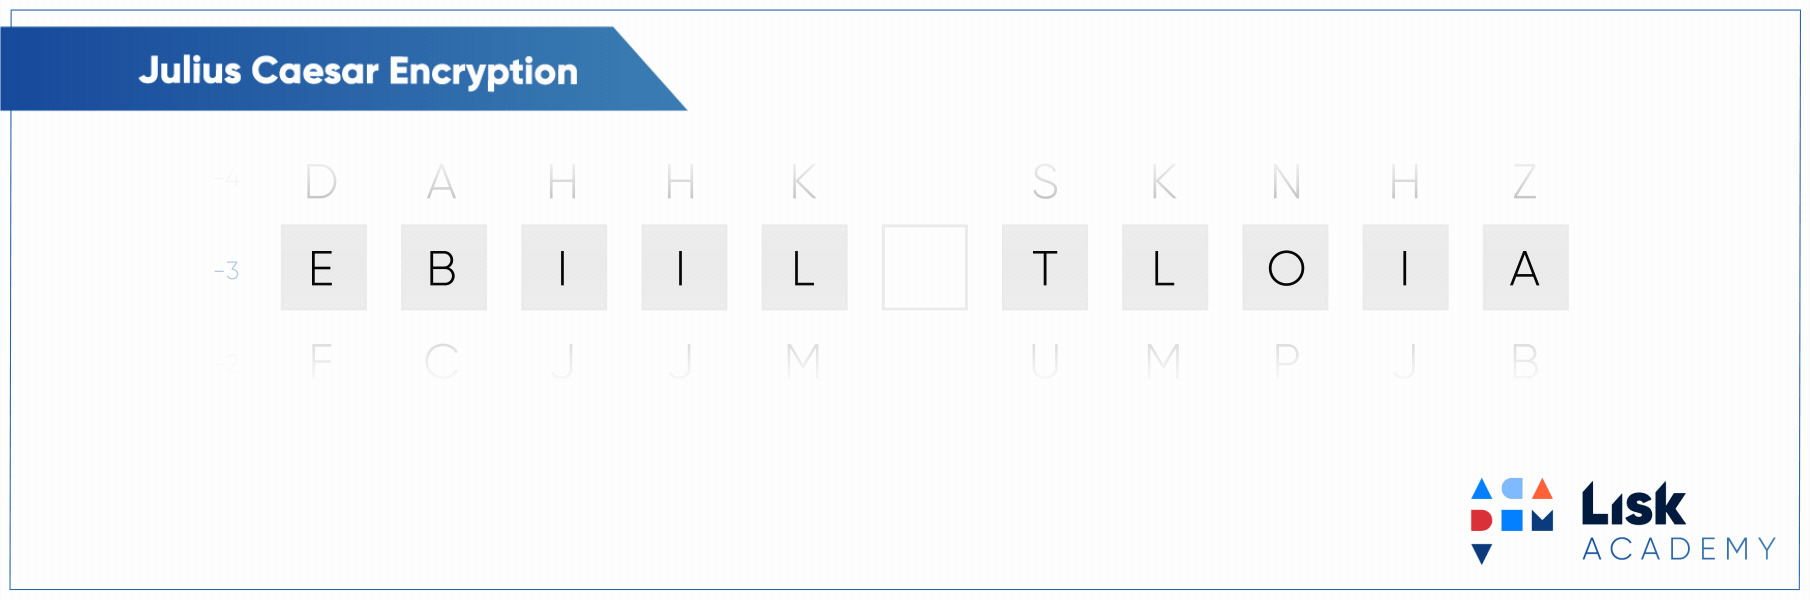
\includegraphics[width=0.9\linewidth]{image/caesarAfter}\label{fig:CaesarAfter}
	\caption{Câu "Hello World" sau khi mã hóa bằng mật mã Caesar}
\end{figure}


Mã nền (codebase) của phần lớn các thuật toán dùng trong mật mã là các dự án mã nguồn mở, nghĩa là code của chúng có thể được xem xét bởi bất kì ai. Thuật toán (cipher) được sử dụng rộng rãi nhất trên thế giới là AES, cho phép bất kì ai đều có thể sử dụng và code của nó được mở để cộng đồng có thể xem. Kết quả là nó đã được nghiên cứu chi tiết và cho đến nay chưa có lỗ hỗng nào được phát hiện.  Thuật toán này cũng được sử dụng bởi NSA, cơ quan tình báo Hoa Kỳ, như một công cụ được chọn để mã hóa thông tin. Vì vậy, có thể nói thông tin được ghi lại trên blockchain được bảo mật với cùng mức độ như bảo mật những bí mật nhạy cảm nhất thế giới. 

Trong blockchain, mật mã được sử dụng chủ yếu cho hai mục đích:
Bảo vệ nhận dạng (identities) của người gửi giao dịch
Đảm bảo các ghi chép trong quá khứ không thể bị giả mạo

Công nghệ blockchain sử dụng mật mã như một phương tiện để bảo vệ nhận dạng của người dùng, đảm bảo giao dịch được thực hiện một cách an toàn và bảo mật mọi thông tin và giá trị lưu trữ. Vì vậy, bất kì ai sử dụng blockchain đều có thể hoàn toàn tự tin rằng thông tin khi đã được ghi trên blockchain thì hoàn toàn hợp lệ và bảo mật.

Mặc dù được xây dựng trên một khuôn khổ tương tự, nhưng mật mã khóa công khai (public-key cryptography), loại mật mã được dùng trong blockchain, phù hợp với các chức năng liên quan đến blockchain hơn so với mật mã khóa đối xứng.

 Public-Key Cryptography, còn được gọi là asymmetric cryptography là một cải tiến trên nền tảng mật mã khóa đối xứng chuẩn: nó cho phép thông tin được truyền nhờ vào một khóa công khai có thể được chia sẽ với bất kỳ ai
 
 Thay vì sử dụng một chìa khóa duy nhất cho cả việc mã hóa và giảm mã, như với trường hợp của mật mã khóa đối xứng, trong mật mã khóa công khai, các chìa khóa riêng rẽ (một khóa công khai và một khóa riêng tư) được sử dụng.
 
 Sự kết hợp giữa khóa công khai và riêng tư của người dùng giúp mã hóa thông tin, còn khóa riêng tư của người nhận và khóa công khai của người gửi giúp giải mã nó. Không thể tìm ra khóa riêng tư dựa trên khóa công khai. Vì vậy, một người dùng có thể gửi khóa công khai của họ đến bất kỳ ai mà không sợ rằng ai đó sẽ có quyền truy cập vào khóa riêng tư của họ. Người gửi có thể mã hóa tập tin và chắc chắn rằng những tập tin đó sẽ chỉ có thể bị giải mã bởi bên được định trước.
 
 Thêm vào đó, thông qua mật mã khóa công khai, một chữ ký điện tử được tạo ra, bảo vệ sự toàn vẹn của dữ liệu. Điều này được thực hiện bằng cách kết hợp chìa khóa riêng tư của người dùng với dữ liệu mà họ muốn kí, thông qua thuật toán nhất định.
 
 Do bản thân dữ liệu là một phần của chữ kí số, hệ thống mạng sẽ không ghi nhận nó là hợp lệ nếu bất kì phần nào của nó bị giả mạo.  Việc chỉnh sửa kể cả nhỏ nhất cũng sẽ làm thay đổi toàn bộ chữ kí, làm cho nó sai khác đi và không dùng được nữa. Thông qua đó, công nghệ blockchain có khả năng đảm bảo rằng bất kì dữ liệu nào đã được ghi vào là đúng, chính xác và không bị giảm mạo. Chữ kí số tạo nên tính bất khả đổi của dữ liệu được khi trong một blockchain.
 
 \section{Chữ kí số}
 
Chữ kí số đúng như tên gọi của nó: nó cung cấp sự xác nhận và chứng thực tương tự như chữ kí bình thường, ở dạng số hóa. Phân đoạn này sẽ thảo luận cách chúng hoạt động cũng như cách đa chữ kí (multisignatures) được sử dụng để tăng thêm một lớp bảo mật.
 
Chữ kí số là một trong những phương tiện chính để đảm bảo tính an toàn và toàn vẹn của dữ liệu được ghi trên một blockchain. Chúng là một bộ phận tiêu chuẩn trong giao thức blockchain, được dùng chủ yếu để bảo vệ giao dịch và khối giao dịch, sự chuyển các thông tin nhạy cảm, phân phối phần mềm, quản lý hợp đồng và các trường hợp khác khi việc phát hiện và ngăn chặn các  hành động làm giả mạo từ bên ngoài. Chữ ký số sử dụng mật mã bất đồng bộ, nghĩa là thông tin có thể được chia sẽ với bất kỳ ai bằng cách sử dụng chìa khóa công khai.
 
 Ở nhiều nơi trên thế giới, chữ ký điện tử có cùng ràng buộc pháp lý như chữ kí thường. Ví dụ về các quốc gia và thực thể  công nhận chúng bao gồm: Liên Minh Châu Âu, Liên Hợp Quốc, Liên Hợp Quốc, Hoa Kỳ, Brazil, Mexico, India, Indonesia, Turkey và Saudi Arabia.
 
 Chữ kí số cung cấp ba lợi thế cho việc lưu trữ và truyền thông tin trên một blockchain. Đầu tiên, chúng đảm bảo tính toàn vẹn. Về lý thuyết, dữ liêụ (đã được mã hóa) được gửi đi tuy không thể bị nhìn thấy nhưng có thể bị thay đổi bởi tin tặc. Tuy nhiên nếu điều này xảy ra, chữ kí của nó cũng sẽ bị thay đổi. Vì vậy dữ liệu đã được kí số không chỉ an toàn do không bị nhìn thấy mà còn tiết lộ nếu nó đã giả mạo.
 
 Chữ kí số không chỉ bảo vệ dữ liệu mà còn bảo vệ nhận dạng của người gửi. Chỉ có chủ nhân của chữ kí số mới nắm và dùng được chữ kí số đó và do đó, một người có thể chắc chắn rằng họ đang liên lạc với người mà họ muốn (liên lạc).
 
 Khi sử dụng công nghệ blockchain, một người dùng có một chìa khóa công khai và một chìa khóa riêng tư, cả hai đều có dạng chuỗi các số và chữ ngẫu nhiên. Có thể coi chìa khóa công khai này, hay đôi khi còn được gọi là địa chỉ công khai, như một địa chỉ email và khóa riêng tư như là mật khẩu. Điều rất quan trọng là không được chia sẻ chìa khóa riêng tư với bất kì ai.
 
 Cuối cùng, chữ kí số mang tính không thể chối bỏ do chìa khóa riêng tư gắn liền với ngươi dùng. Điều này có nghĩa là nếu cái gì đó đã được kí số bởi một người dùng, nó đã được ràng buộc về mặt pháp lý và hoàn toàn liên kết với cá nhân đó. Như đã chỉ ra ở trên, điều này phụ thuộc nhiều vào không có nghi ngờ về việc chìa khóa riêng tư dùng để kí dữ liệu không bị xâm phạm, sử dụng và nhìn thấy bởi bất kỳ ai ngoài chủ sở hữu của nó. 
 
 Mỗi người có một chữ kí duy nhất và nó được tạo ra bằng cách sử dụng ba thuât toán sau:
 \begin{itemize}
   \item  Một thuật toán tạo chìa khóa, cung cấp một chìa khóa công khai và một chìa khóa riêng tư.
 \item Một thuật toán kí giúp kết hợp dữ liệu và khóa riêng tư để tạo thành một chữ kí
 \item Một thuật toán giúp xác thực chữ kí và xác định xem tin nhắn đó có đáng tin hay không dựa trên tin nhắn, khóa công khai và chữ kí.
 \end{itemize}

 
 Tính năng quan trọng nhất của những thuật toán đó là:
\begin{itemize}
   \item Khiến việc tạo ra khóa riêng tư dựa trên khóa công khai hoặc dữ liệu mà nó mã hóa trở nên bất khả thi.
 \item Đảm bảo tính xác thực của một chữ kí dưạ trên tin nhắn và khóa riêng tư, được  xác thực thông qua khóa công khai.
 \end{itemize} 
 
 \subsection{Đa chữ kí}
 Đa chữ ký (Multisignature), đôi khi được rút ngắn thành multisig, là một chương trình chữ kí số đòi hỏi nhiều hơn một người kí để một giao dịch được chấp thuận. Khái niệm về hệ thống đa chữ kí không phải được tạo ra chỉ để dùng cho tiền ảo mà đã xuất hiện từ hàng ngàn năm trước.  Những tu sĩ ở núi Athos đã bảo vệ hầm mộ của nó với nhiều chìa khóa và cần nhiều hơn một chìa để mở khóa hầm mộ. Điều này có nghĩa là không một tu sĩ đơn lẻ nào có thể tiếp cập các di tích quý giá mà không cần ít nhất một tu sĩ khác.
 
Multisig được sử dụng bởi nhiều loại tiền ảo, bao gồm Bitcoin\footnote{Đồng tiền ảo mã nguồn mở, phi tập trung đầu tiên thành công chạy trên một mạng ngang hàng (P2P)} và List, như một phương tiện để cải thiện độ bảo mật cũng như chia khả năng đưa ra quyết định cho nhiều hơn một bên. 
%Dạng gửi giao dịch qua đồng LSK\footnote{Đơn vị tiền của List} này giúp hệ thống an toàn hơn trước tin tặc cũng như bất kì ai tình cờ có  được quyền truy cập vào cụm mật khẩu ( passphrase\footnote{Tương tự như mật khẩu, chúng đều hoạt động như chứng chỉ đăng nhập của người dùng}) của người dùng Lisk.
 
 Ví dụ, với đa chữ kí ta có thể tạo một dịch vụ giao kèo 2 trên 3, nghĩa là để xác nhận một giao dịch đòi hỏi cần phải có sự chấp nhận của hai trong số ba bên để thực hiện. Một ví dụ về trường hợp đa chữ kí hữu ích là tài khoản tiết kiệm cho một đứa trẻ, khi cả đứa trẻ và ít nhất một trong số bố mẹ nó cần đồng thuận cách tiền trong đó được rút ra và xài. Nó cũng mở ra tùy chọn mà các quyết định quan trọng được đưa ra chỉ từ phía phụ huynh, miễn là cả hai đều đồng ý.
 
Chữ kí số là thành phần tối quan trọng trong việc bảo vệ dữ liệu trên một blockchain\comment{, cũng như nút là nền tảng để xây dựng nên hệ thống mạng chứa blockchain}.

\section{Nút}
\subsection{Khái niệm về nút}

Một nút là một thiết bị trên một hệ thống mạng blocchain, và về bản chất chính là nền tảng của công nghệ này: nó giúp blockchain hoạt động và tồn tại. \underline{Các nút được phân bố trên một mạng lưới rộng khắp và thực hiện nhiều tác vụ khác nhau.}

Một nút có thể là một thiết bị điện tử bất kỳ, bao gồm máy tính, điện thoại hoặc thậm chí là máy in, miễn là nó được kết nối với Internet và do đó có một địa chỉ IP. Vai trò của một nút là hỗ trợ hệ thống mạng bằng cách duy trì một bản sao của blockchain và trong một số trường hợp, giúp xử lí các giao dịch. Nút thường có dạng cấu trúc cây nhị phân. Mỗi loại tiền ảo có nút của riêng nó, duy trì các bản ghi chép giao dịch của đồng tiền đó. 

Các nút là những thành phần đơn lẻ của một cấu trúc lớn hơn: blockchain. Chủ sở hữu của các nút  sẵn sàng đóng góp tài nguyên tính toán của họ để lưu trữ và xác thực các giao dịch và do đó họ có cơ hội nhận được phí giao dịch và nhận phần thưởng cho công việc ấy. 

Việc xử lý các giao dịch đòi hỏi một lượng lớn sức mạnh tính toán và xử lý, nghĩa là năng lực của một máy tính bình thường không đáp ứng yêu cầu. Generally, professional miners tend to invest in extremely powerful computing devices known as CPUs (central processing units) or GPUs (graphics processing units) in order to keep up with the demand for processing power that is required for them to validate transactions and as such earn the rewards that comes with doing so.




 
 
 
 
  
 
 
